Der Aufbau ist bereits fertig konfiguriert. Die Ausgangssignale beider Detektoren werden mit dem Oszilloskop betrachtet und anschließend die nötigen Spektren aufgenommen. 

\subsection{Szintillationsspektrometer}
Zunächst wird das Signal des Szintillationsdetektors direkt am Augang des Vorverstärkers des Photomultipliers auf dem Oszilloskop betrachtet. Das Signal ist in Abbildung \ref{fig:szint_nach_vorv} zu sehen.
\begin{figure}[h]
  \centering
  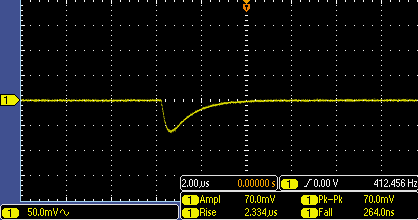
\includegraphics[width=0.5\textwidth]{data/raw/szint_nach_vorv.png}
  \caption{Szintillatorsignal nach Vorverstärker}
  \label{fig:szint_nach_vorv}
\end{figure}

Das Signal steigt schnell in etwa \SI{0.6}{\micro\second} an und fällt danach über eine Zeit von etwa \SI{3.5}{\micro\second} exponentiell ab. Der exponentielle Abfall entsteht durch den exponentiellen Zerfall der angeregten Zustände im Szintillator zum Grundzustand.\\

Das Signal nach dem Hauptverstärker wird mit dem Oszilloskop aufgenommen (Abbildung \ref{fig:szint_nach_haupt}). Neben der Verstärkung des Signals hat sich auch die Form verändert. Anstiegs- und Abfallszeit habne sich in etwa verdoppelt. Außerdem wechselt das Signal während des Abfalls die Polarität. Insgesamt ähnelt das Signal einer gedämpften Schwingung.\\ 
\begin{figure}[h]
  \centering
  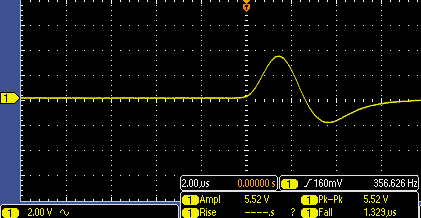
\includegraphics[width=0.5\textwidth]{data/raw/szint_nach_haupt.png}
  \caption{Szintillatorsignal nach Hauptverstärker}
  \label{fig:szint_nach_haupt}
\end{figure}

Mit dem Aufnahmeprogramm des Computers werden ein Untergrundspektrum sowei die Spektren von $^{60}$Co, $^{137}$Cs und $^{152}$Eu aufgenommen. Es ist darauf zu achten, dass die Proben immer im gleichen Abstand von \SI[separate-uncertainty = true]{4.5(5)}{\centi\meter} zum Detektor platziert werden.

\subsection{Ge-Halbleiterdetektor}
Mit dem Halbleiterdetektor werden wieder die Signale nach Vor- und Hauptverstärker oszilloskopiert. In Abbildung \ref{fig:ge_nach_vorv} ist das Signal nach dem Vorverstärker zu sehen. Das Signalstärke übertrifft bereits ohne Hauptverstärker das Signal des Szintillationsdetektors nach dem Hauptverstärker.
Der Signalform ist äquivalent zum Szintillationsdetektor. 
\begin{figure}[h]
  \centering
  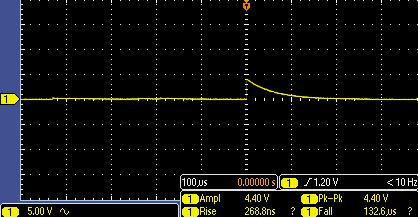
\includegraphics[width=0.5\textwidth]{data/raw/ge_nach_vorv.png}
  \caption{Halbleiterdetektorsignal nach Vorverstärker}
  \label{fig:ge_nach_vorv}
\end{figure}

Auch die Aufnahme nach dem Hauptverstärker (Abbildung \ref{fig:ge_nach_haupt}) zeigt qualitativ den gleichen Verlauf wie beim Szintillationsdetektor nach dem Hauptverstärker. Die Anstiegs- und Abfallszeit ist beim Germaniumdetektor allerdings mehr als doppelt so lang wie beim Siliziumdetektor. Es ist zu sehen, dass die Abfallszeit durch den Hauptverstärker verringert wird.
\begin{figure}[h]
  \centering
  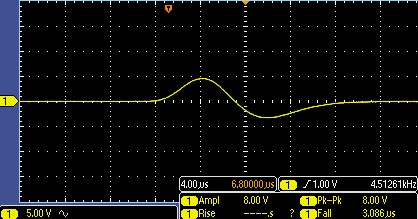
\includegraphics[width=0.5\textwidth]{data/raw/ge_nach_haupt.png}
  \caption{Halbleiterdetektorsignal nach Hauptverstärker}
  \label{fig:ge_nach_haupt}
\end{figure}

Wieder werden ein Untergrundspektrum sowei die Spektren von $^{60}$Co, $^{137}$Cs und $^{152}$Eu aufgenommen. Der Abstand zum Detektor beträgt nun jeweils \SI[separate-uncertainty = true]{7.0(5)}{\centi\meter}

\subsection{Langzeitmessungen}
In zwei Langzeitmessungen (jeweils über etwa einen Tag) werden mit dem Halbleiterdetektor ein Untergrundspektrum und das Spektrum einer Bodenprobe aufgenommen. Bei beiden Messungen wird Blei zur Abschirmung des Untergrundes verwendet.
